\taskpic{ Однородный массивный уголок с одинаковыми сторонами длины
  $2R$ каждая закреплён в вертикальной плоскости. В него вставлен шар
  радиуса $R$. При каком коэффициенте трения между шаром и уголком
  система будет находиться в равновесии?}
{
  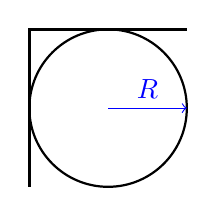
\begin{tikzpicture}
    \draw[very thick] (0,0) -- (0,2) -- (2,2);
    \draw[thick] (1,1) circle (1cm);
    \draw[blue,->] (1,1) -- (2,1) node[midway,above] {$R$};
  \end{tikzpicture}
}
% TPT, dec 2013